% Intended LaTeX compiler: xelatex
\documentclass[aspectratio=64,12pt]{beamer}
\usepackage{graphicx}
\usepackage{longtable}
\usepackage{wrapfig}
\usepackage{rotating}
\usepackage[normalem]{ulem}
\usepackage{amsmath}
\usepackage{amssymb}
\usepackage{capt-of}
\usepackage{hyperref}
\institute{Università di Siena}
\usepackage{localheader}
\usepackage{tikz}
\usepackage{booktabs,tabularx,tabularray}
\usepackage{setspace}
\usepackage{quoting}
\usepackage[italian]{babel}
\usepackage{fancybox}
\usepackage{tabularray}
\newcolumntype{R}{>{\raggedleft\arraybackslash}X}
\newenvironment{nobulletlist}{\begin{list}{--}{\itemsep=3pt\itemindent=2ex\labelsep=.7ex\leftmargin=0pt}}{\end{list}}
\usetheme{default}
\author{Massimo D'Antoni}
\date{2024-2025}
\title{Il ruolo economico dello Stato}
\subtitle{Scienza delle Finanze}
\hypersetup{
 pdfauthor={Massimo D'Antoni},
 pdftitle={Il ruolo economico dello Stato},
 pdflang={Italian}}
\begin{document}

\maketitle

\section{Un quadro generale dell'intervento pubblico}


%%%%%%%%%%%%%%%%%%%%%%%%%%%%%%%%%%%%%%%%%%%%
\begin{frame}{Il ruolo economico dello Stato}
\begin{itemize}
\item L'operatore pubblico (lo Stato, con le sue articolazioni territoriali)
interviene nell'attività economica con molteplici modalità:
\begin{itemize}
\item definizione e garanzia dell'esercizio di diritti individuali
(es. proprietà, integrità fisica)
\item divieti e obblighi di fare (es. standard di sicurezza)
\item controllo per via proprietaria di attività produttive (società
partecipate) o regolazione di attività private (es. servizi di trasporto)
\item produzione diretta di beni e servizi (scuole, ospedali)
\item trasferimenti monetari (pensioni, sussidi)
\item imposizione fiscale (IVA, imposte sul reddito)
\end{itemize}
\item Cosa giustifica tale intervento? Quali criteri per valutarne la bontà?
\item Alcune modalità – ma non tutte – si riflettono nella contabilità dello Stato
come entrate (imposte) e uscite (spesa pubblica)
\end{itemize}
\end{frame}

%%%%%%%%%%%%%%%%%%%%%%%%%%%%%%%%%%%%%%%%%%%%
\begin{frame}{Il peso dello stato dal punto di vista quantitativo}
\begin{itemize}
\item Nelle definizioni adottate internazionalmente l’aggregato rilevante è la \alert{Pubblica Amministrazione}.
\item Ai fini della Contabilità nazionale (ESA2010) guardiamo alla natura dell’attività
svolta:
\end{itemize}
\begin{quoting}
«Le Amministrazioni pubbliche sono l’insieme delle unità che producono beni e
servizi non destinabili alla vendita o la cui funzione principale consiste
nella redistribuzione del reddito e della ricchezza del paese.»
\end{quoting}
\begin{itemize}
\item Indipendentemente dal regime giuridico (pubblico o privato),
per essere classificata nel settore delle P.A., un'unità istituzionale:
\begin{itemize}
\item deve essere di proprietà o amministrata o controllata da Amministrazioni pubbliche;
\item non deve vendere sul mercato o deve vendere a prezzi non economicamente
rilevanti (criterio: i ricavi non devono eccedere il 50\% dei costi di
produzione dei servizi)
\end{itemize}
\end{itemize}
\end{frame}

%%%%%%%%%%%%%%%%%%%%%%%%%%%%%%%%%%%%%%%%%%%%
\begin{frame}{I tre sottosettori della P.A. secondo la contabilità nazionale}
\begin{itemize}
\item La dimensione della P.A. si può apprezzare prendendo in considerazione il
bilancio consolidato degli enti che ne sono parte
\item L'aggregato Pubbliche Amministrazioni comprende:
\begin{itemize}
\item le \alert{Amministrazioni centrali}: organi amministrativi dello Stato e enti
centrali con competenza nazionale (enti di ricerca, enti di regolazione,
ecc.), esclusi enti previdenziali;
\item le \alert{Amministrazioni locali}: Regioni e province autonome, Province, Comuni,
ASL e aziende ospedaliere, università, enti per il diritto allo studio,
enti parco, comunità montane, camere di commercio, ecc.;
\item gli \alert{Enti previdenziali}: erogano prestazioni sociali obbligatorie (Inps,
Inail, Inpdap, altre Casse previdenziali ecc).
\end{itemize}
\end{itemize}

\begin{block}{}
\footnotesize
→ L'ISTAT redige ogni anno un \href{https://www.istat.it/it/archivio/190748}{elenco delle unità istituzionali appartenenti
alla P.A.}\\[0pt]
(vedi in particolare la Nota esplicativa)
\end{block}
\end{frame}

%%%%%%%%%%%%%%%%%%%%%%%%%%%%%%%%%%%%%%%%%%%%
\begin{frame}{I principali enti nei tre sottosettori della P.A.}
\vspace*{-5mm}
\fontsize{8}{8.5}\selectfont
\begin{columns}[t]
\begin{column}{.33\columnwidth}
\begin{block}{\footnotesize Amministrazioni centrali}
\begin{nobulletlist}
\item Gli organi costituzionali e di rilievo costituzionale, la Presidenza del Consiglio dei Ministri e i Ministeri;
\item le agenzie fiscali (ad es. Agenzia del Demanio, Agenzia delle Entrate);
\item gli enti di regolazione dell’attività economica (ad es. Agenzia italiana del farmaco e Ispettorato nazionale del lavoro);
\item gli enti produttori di servizi economici (ad es. Anas, Ente per l’aviazione civile, Equitalia, Fintecna, Rete Ferroviaria Italiana);
\item le autorità amministrative indipendenti (ad es. authority dei trasporti, della concorrenza);
\item gli enti produttori di servizi assistenziali, ricreativi e culturali (ad es. Croce Rossa italiana, CONI, RAI);
\item gli enti e istituzioni di ricerca (ad es. CNR, INFN, Istituto superiore di sa\-nità).
\end{nobulletlist}
\end{block}
\end{column}

\begin{column}{.33\columnwidth}
\begin{block}{\footnotesize Amministrazioni locali}
\begin{nobulletlist}
\item le Regioni e province autonome, le province e città metropolitane, i comuni, le comunità montane, le unioni di comuni;
\item le Agenzie territoriali (ad es. per il diritto allo studio universitario, per il turismo, le agenzie de lavoro, le agenzie regionali e provinciali per la formazione, la ricerca e l’ambiente) e altre agenzie regionali e locali;
\item le aziende sanitarie locali, le aziende ospedaliere;
\item le camere di commercio;
\item i consorzi tra amministrazioni locali;
\item i parchi nazionali e gli enti gestori di parchi e aree protette;
\item le fondazioni lirico-sinfoniche, i teatri nazionali e di rilevante interesse culturale;
\item le università e istituti di istruzione universitaria pubblici.
\end{nobulletlist}
\end{block}
\end{column}

\begin{column}{.33\columnwidth}
\begin{block}{\footnotesize Enti di previdenza}
\begin{nobulletlist}
\item INPS (Istituto nazionale previdenza sociale);
\item l’INAIL, Istituto nazionale per l’assicurazione contro gli infortuni sul la\-voro;
\item casse di previdenza e assistenza per specifiche categorie professio\-nali.
\end{nobulletlist}
\end{block}
\end{column}
\end{columns}
\end{frame}

%%%%%%%%%%%%%%%%%%%%%%%%%%%%%%%%%%%%%%%%%%%%
\begin{frame}{Quanta parte del PIL è prodotto dalla P.A.?}

\begin{figure}
\centering
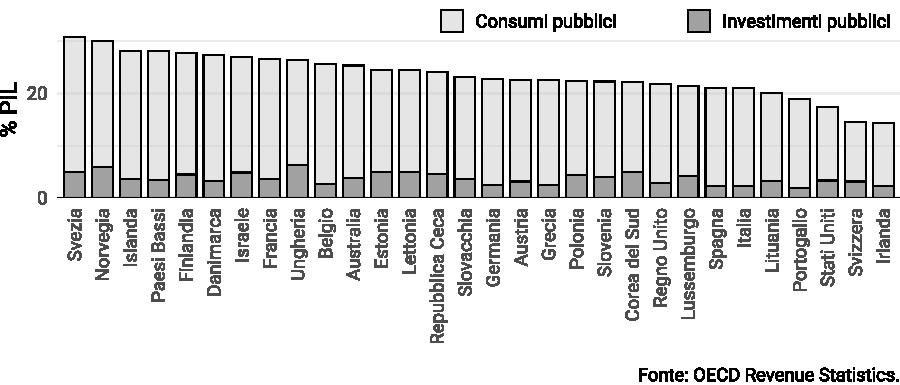
\includegraphics[width=.9\textwidth]{./figure/consumi-investimenti-pubblici-PIL.pdf}
\end{figure}

\begin{itemize}
\item Nelle economie avanzate, la quota del PIL rappresentata da consumi e
investimenti pubblici è generalmente compresa tra il 20 e il 30\%
\end{itemize}

\end{frame}


%%%%%%%%%%%%%%%%%%%%%%%%%%%%%%%%%%%%%%%%%%%%
\begin{frame}{Il livello complessivo di spesa pubblica}
\begin{columns}
\begin{column}{.6\columnwidth}
\begin{itemize}
\item La spesa pubblica non comprende solo la produzione e acquisto di beni e
servizi (conteggiati nel PIL come consumi e investimenti pubblici),
ma anche la spesa per trasferimenti (ad es. le pensioni) che vanno ad
alimentare la domanda privata di beni e servizi.

\item Il totale delle spese della P.A. in Italia è stato pari a:
\begin{itemize}
\item 871 mld nel 2019, pari al 48,5\% del PIL
\item 947 mld nel 2020, pari al 57\% del PIL
\item 1.026 mld nel 2021, pari al 56,3\% del PIL
\item 1.092 mld nel 2022, pari al 56,1\% del PIL
\end{itemize}
\end{itemize}
\end{column}

\begin{column}{.4\columnwidth}
\begin{resize}{.9}
\begin{block}{}
\footnotesize
La spesa può aumentare in valore assoluto ma ridursi in rapporto al PIL
\end{block}

\begin{block}{}
  \footnotesize I valori riportati sono diversi da quelli nel testo, in quanto
  vengono continuamente aggiornati e spesso corretti dall’ISTAT.  I dati
  riferiti agli anni più recenti sono da considerare sempre provvisori e a
  volte anche i dati più lontani nel tempo cambiano, per effetto dell’adozione
  di nuovi criteri di misura e classificazione
\end{block}

\begin{block}{}
\footnotesize
Convenzionalmente, per consentire confronti tra paesi e nel tempo, si rapporta la spesa al PIL, ma queste percentuali \alert{non significano} che il PIL è per il 55\% pubblico e per il restante 45\% privato!
\end{block}
\end{resize}
\end{column}
\end{columns}
\end{frame}

%%%%%%%%%%%%%%%%%%%%%%%%%%%%%%%%%%%%%%%%%%%%
\begin{frame}{La classificazione economica della spesa pubblica}
Possiamo classificare la spesa in base alla categoria economica:
\begin{columns}
\begin{column}{.6\columnwidth}
\begin{figure}
\centering
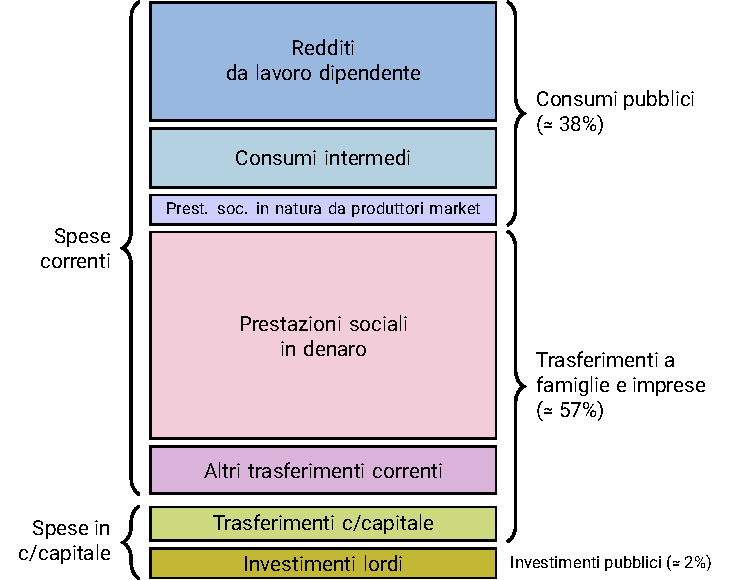
\includegraphics[width=1.1\textwidth]{./figure/spesa-pubblica-classificazione-economica-color.pdf}
\end{figure}
\end{column}

\begin{column}{.4\columnwidth}
\footnotesize
\begin{itemize}
\item spese correnti e in conto capitale;
\item distinguiamo i consumi pubblici (misurati dalle spese necessarie per gli input, lavoro e altri input produttivi) dai trasferimenti ad altri soggetti;
\item sono spesa per consumi anche gli acquisti di beni e prestazioni da fornitori privati a beneficio dei cittadini (es. molte prestazioni sanitarie);
\item in Italia il 60\% circa della spesa pubblica è rappresentato da trasferimenti.
\end{itemize}
\end{column}
\end{columns}
\end{frame}

%%%%%%%%%%%%%%%%%%%%%%%%%%%%%%%%%%%%%%%%%%%%
\begin{frame}{La classificazione funzionale della spesa pubblica}
\begin{resize}{.9}  
Possiamo classificare la spesa in base alla funzione svolta:

\begin{columns}
\begin{column}{.6\columnwidth}
\begin{figure}
\centering
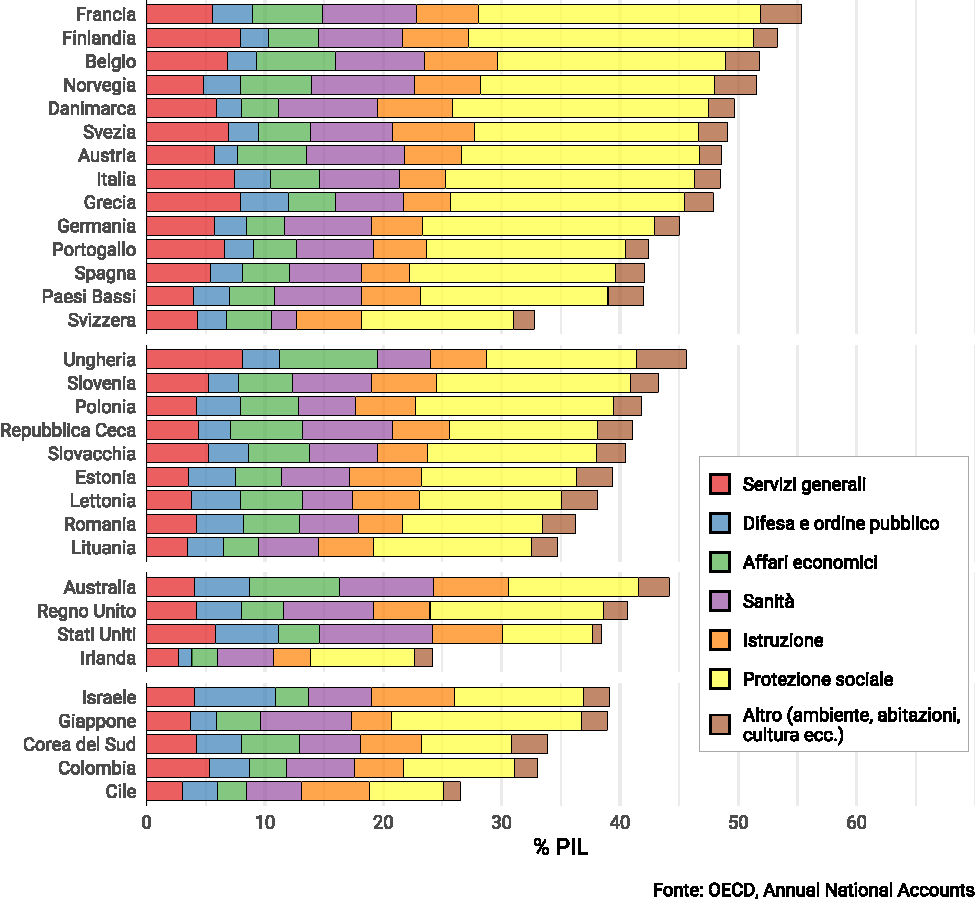
\includegraphics[width=\textwidth]{./figure/spesa-pubblica-per-funzioni-2019-orizz-color.pdf}
\end{figure}
\end{column}

\begin{column}{.4\columnwidth}
\footnotesize
\begin{enumerate}
\item Servizi generali delle P.A.
\item Difesa
\item Ordine pubblico e sicurezza
\item Affari economici
\item Protezione dell’ambiente
\item Abitazioni e assetto territoriale
\item Sanità
\item Attività ricreative, culturali e di culto
\item Istruzione
\item Protezione sociale
\end{enumerate}
Le funzioni 1-6 sono consumi collettivi, 7-10 sono consumi individuali (in 8 sia individuali che collettivi)
\end{column}
\end{columns}
\end{resize}
\end{frame}

%%%%%%%%%%%%%%%%%%%%%%%%%%%%%%%%%%%%%%%%%%%%
\begin{frame}{La classificazione funzionale della spesa pubblica /2}
\begin{figure}
\centering
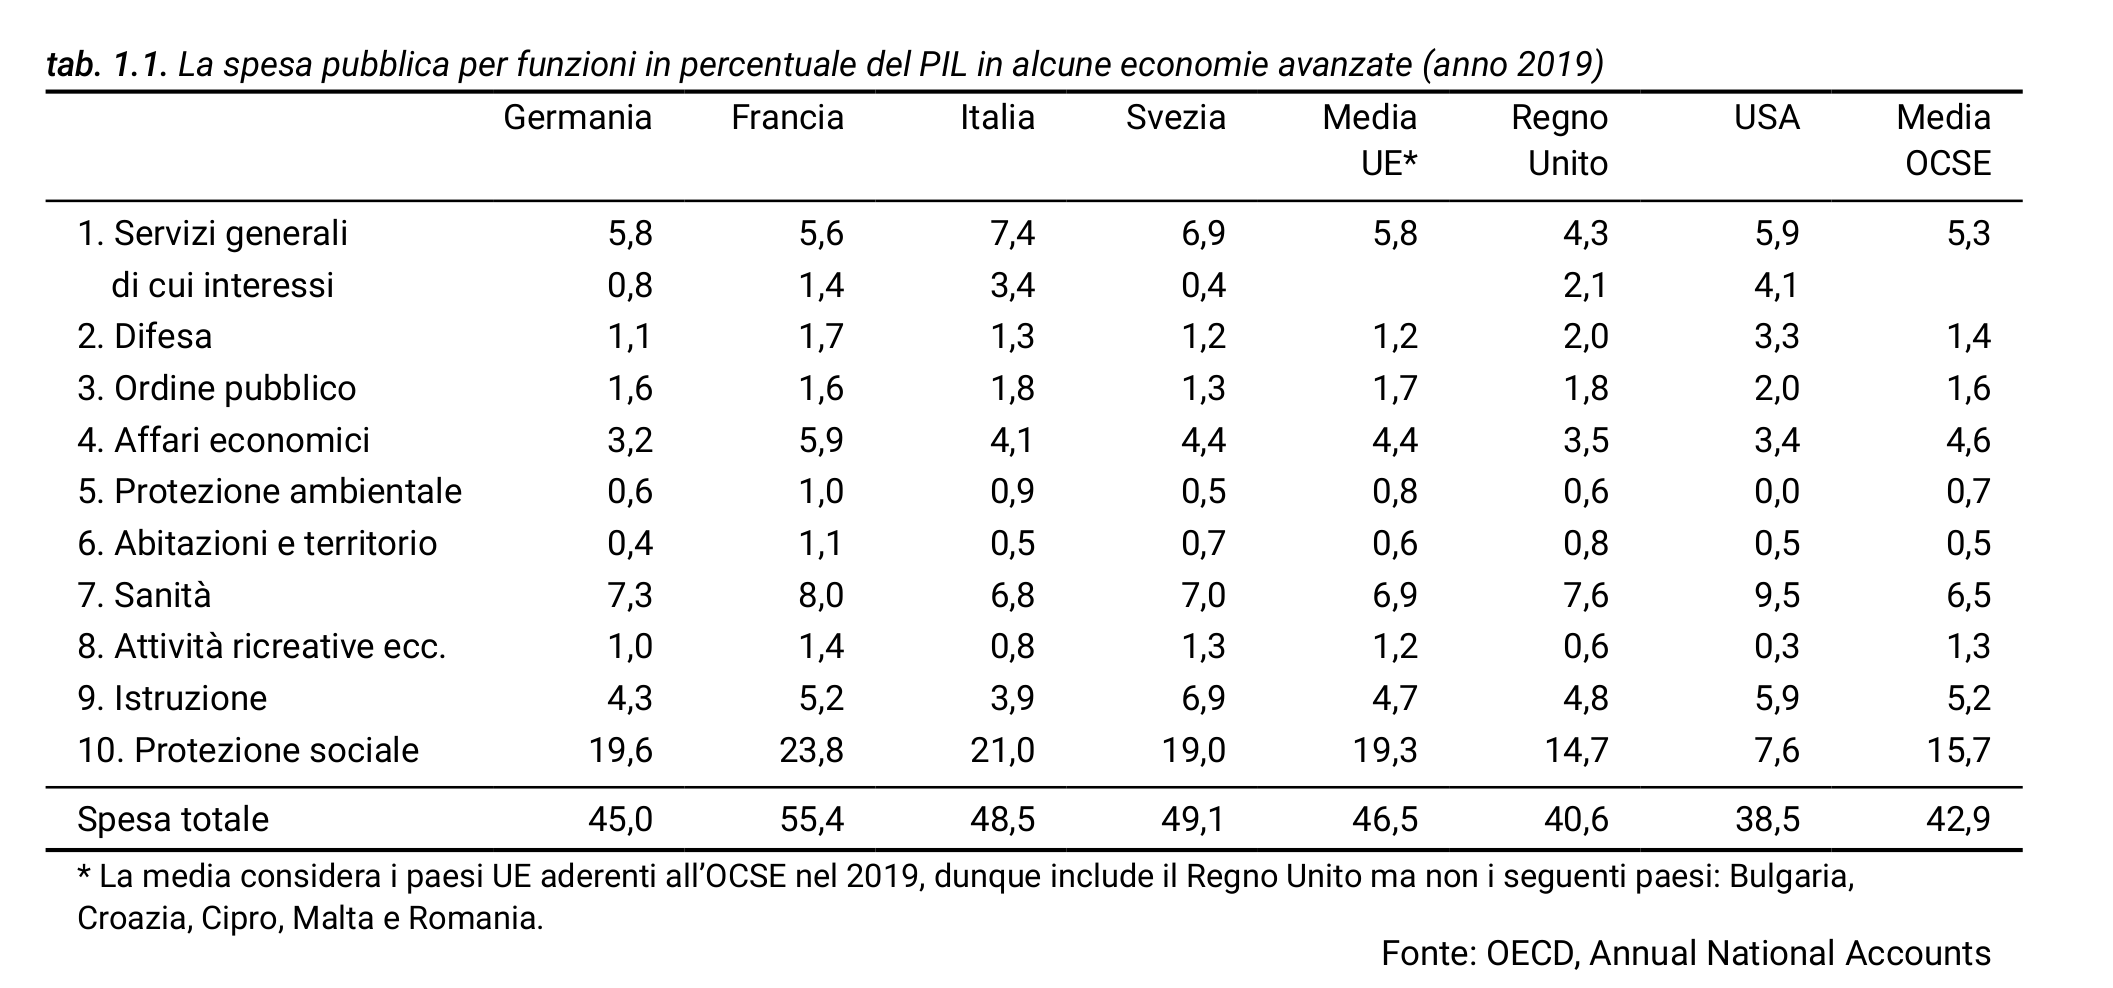
\includegraphics[width=\textwidth]{./figure/tab-1-1.png}
\end{figure}

\footnotesize
\begin{itemize}
\item Osserviamo la rilevanza della spesa per interessi nella funzione servizi generali (in Italia ma anche negli USA)
\item La spesa al netto della spesa per interessi è detta \alert{spesa primaria}
\end{itemize}
\end{frame}

%%%%%%%%%%%%%%%%%%%%%%%%%%%%%%%%%%%%%%%%%%%%
\begin{frame}{Funzioni e categorie insieme}
\begin{itemize}
\item La tipologia di spesa (personale, trasferimenti, ecc.) può essere molto diversa a seconda della funzione
\end{itemize}

\begin{center}
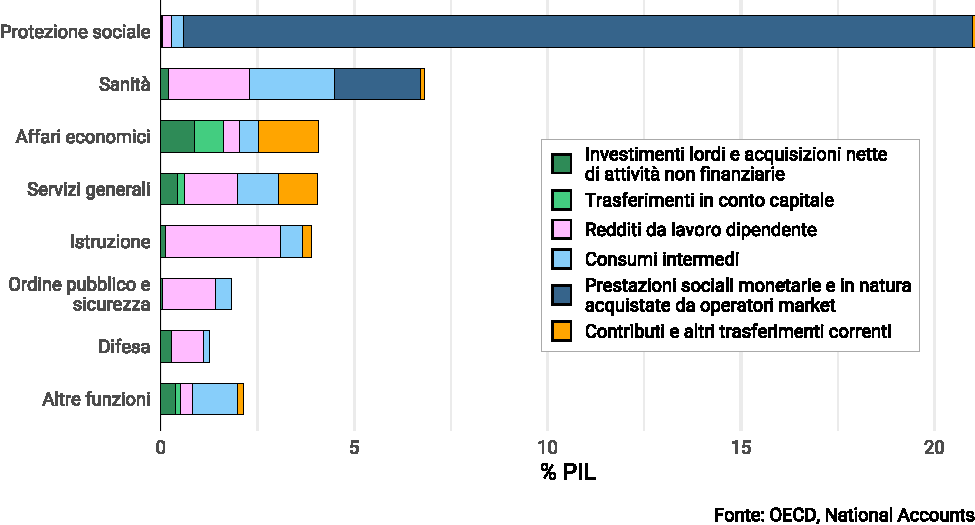
\includegraphics[height=5cm]{./figure/spesa-primaria-funzioni-categorie-ITA-color.pdf}
\end{center}

\vspace{-5mm}
\begin{columns}
\begin{column}{.33\columnwidth}
\begin{block}{}
\footnotesize\flushleft
La spesa per protezione sociale è prevalentemente data da trasferimenti
\end{block}
\end{column}

\begin{column}{.33\columnwidth}
\begin{block}{}
\footnotesize\flushleft
Per istruzione, ordine pubblico e difesa prevalgono le spese per personale
\end{block}
\end{column}

\begin{column}{.33\columnwidth}
\begin{block}{}
\footnotesize\flushleft
Nella sanità e nei servizi generali sono molto rilevanti i consumi intermedi
\end{block}
\end{column}
\end{columns}
\end{frame}

%%%%%%%%%%%%%%%%%%%%%%%%%%%%%%%%%%%%%%%%%%%%
\begin{frame}{Qualche avvertenza}
\begin{itemize}
\item La spesa della P.A. fornisce una visione parziale dell’entità dell’intervento pubblico:
\begin{itemize}
\item alcune forme di intervento pubblico non si traducono in entrate e uscite (ad es. obblighi di assicurazione);
\item in sistemi diversi, interventi con effetti equivalenti posso assumere la forma di una spesa, o di una minore entrata (ad es. tax expenditure);
\item dalla spesa pubblica non registra la presenza dello Stato nei mercati in cui si vendono beni e servizi (società partecipate).
\end{itemize}
\item Parlare di «spesa pubblica» in generale vuol dire considerare in modo unitario fenomeni diversificati, che hanno una varietà di giustificazioni e possono presentare problematiche molto diverse.
\end{itemize}
\end{frame}

%%%%%%%%%%%%%%%%%%%%%%%%%%%%%%%%%%%%%%%%%%%%
\begin{frame}{L'evoluzione della spesa pubblica nel tempo}
\begin{figure}
\centering
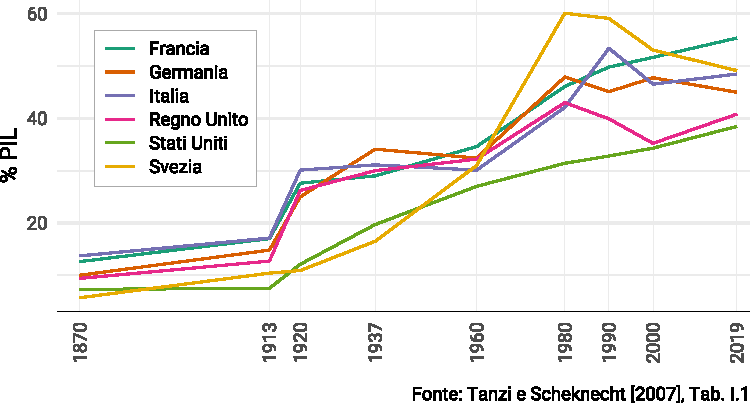
\includegraphics[width=\textwidth]{./figure/hist-government-expenditure-tanzi-scheknecht-color.pdf}
\end{figure}
\end{frame}

%%%%%%%%%%%%%%%%%%%%%%%%%%%%%%%%%%%%%%%%%%%%
\begin{frame}{La crescita storica della spesa pubblica: spiegazioni}
\begin{resize}{.9}
\begin{columns}
\begin{column}{.5\columnwidth}
\begin{block}{Adolph Wagner\newline\footnotesize \emph{Finanzwissenschaft} (1877)}
\footnotesize
Rilevò una tendenza alla crescita dell’intervento pubblico («Legge dell’aumento dell’attività dello Stato», poi nota come «Legge di Wagner»):
\begin{itemize}
\item La crescita della complessità della società, l’industrializzazione, l’urbanizzazione, creano una domanda di protezione sociale e di regolazione delle attività economiche;
\item la crescita del reddito incoraggia l’espansione di certe spese che il mercato non è in grado di fornire in misura adeguata;
\item la necessità di adottare nuove tecnologie e la scala degli investimenti richiesti (es. ferrovie) richiede l’azione dello Stato.
\end{itemize}
\end{block}
\end{column}
\begin{column}{.5\columnwidth}
\begin{block}{Francesco Saverio Nitti\newline\footnotesize (\emph{La scienza delle finanze}, 1903, 1936)}
\footnotesize
\begin{itemize}
\item L’aumento delle spese militari dovuto alla ricerca di supremazia politica e imperialismo, con armi sempre più sofisticate e costose;
\item i grandi lavori pubblici necessari per sfruttare tecnologie quali il motore a vapore e l’elettricità;
\item la prevenzione dei mali sociali nel campo dell’igiene e la sanità;
\item la partecipazione delle classi popolari alla vita pubblica, che ha spinto a sviluppare certi servizi prima non ritenuti di utilità sociale.\\[0pt]
Una tendenza che osserviamo non solo nelle democrazie, ma anche nei regimi dispotici.
\end{itemize}
\end{block}
\end{column}
\end{columns}
\end{resize}
\end{frame}

%%%%%%%%%%%%%%%%%%%%%%%%%%%%%%%%%%%%%%%%%%%%
\begin{frame}{La crescita storica della spesa pubblica: spiegazione /2}
\begin{itemize}
\item Effetto delle trasformazioni economiche e sociali:
\begin{itemize}
\item urbanizzazione e mobilità geografica;
\item l’aumento della speranza di vita;
\item il cambiamento tecnologico;
\item l’aumento della partecipazione femminile alla forza lavoro;
\item la crescente globalizzazione e apertura delle economie ai mercati internazionali.
\end{itemize}
\item Mutamenti nelle preferenze individuali:
\begin{itemize}
\item l’aumento del reddito ha aumentato la natura di beni «superiori» (elasticità rispetto al reddito $> 1$), spesso  consumati collettivamente
\item le comunicazioni diffondono rapidamente stili di vita e domanda di servizi forniti in altre regioni e paesi.
\end{itemize}
\end{itemize}
\end{frame}

%%%%%%%%%%%%%%%%%%%%%%%%%%%%%%%%%%%%%%%%%%%%
\begin{frame}{La crescita storica della spesa pubblica: spiegazione /3}
\begin{itemize}
\item È aumentata la capacità di reperire risorse attraverso la tassazione:
\begin{itemize}
\item l’aumento della dimensione di impresa con lo sviluppo di tecniche di amministrazione e contabilità;
\item l’affidamento di una quota crescente di servizi al mercato ha ampliato il volume delle transazioni monetarie.
\end{itemize}
\item Mutamenti nel livello di tassazione percepito come accettabile:
\begin{itemize}
\item innalzamento dei redditi al di sopra del livello della sussistenza;
\item la democratizzazione ha favorito il riconoscimento della legittimità delle spese dello Stato.
\end{itemize}
\item L’idea che il livello «tollerabile» di imposte possa essere modificato e progressivamente innalzato:
\begin{itemize}
\item Peacock e Wiseman considerano l’effetto di eventi eccezionali (guerre e gravi crisi economiche);
\item per Bird l’adattamento ad aumenti e riduzioni di spesa è asimmetrico.
\end{itemize}
\end{itemize}
\end{frame}


%%%%%%%%%%%%%%%%%%%%%%%%%%%%%%%%%%%%%%%%%%%%
\begin{frame}{La crescita storica della spesa pubblica: spiegazione /4}
\begin{itemize}
\item Per Baumol, l’aumento della spesa dipende dall’effetto combinato di:
\begin{itemize}
\item differenziale nella dinamica della crescita della produttività tra settori;
\item domanda rigida per i beni prodotti nei settori a bassa dinamica di produttività;
\item lo Stato può sostenere alcuni beni diventati particolarmente costosi (es. musica dal vivo, teatro)
\item i beni e servizi dello Stato possono essere concentrati in settori caratterizzati da minore crescita della produttività (es. servizi di cura)
\end{itemize}
\item Se la domanda non è rigida l’«Effetto Baumol» o «Baumol desease» spiega la sparizione di settori tradizionali.
\end{itemize}
\end{frame}

%%%%%%%%%%%%%%%%%%%%%%%%%%%%%%%%%%%%%%%%%%%%
\begin{frame}{La crescita della spesa pubblica: chi ha ragione?}
\begin{itemize}
\item È probabilmente inutile cercare «la» spiegazione corretta: certe spiegazioni valgono per alcune categorie di spesa ma non per altre.
\end{itemize}

\begin{center}
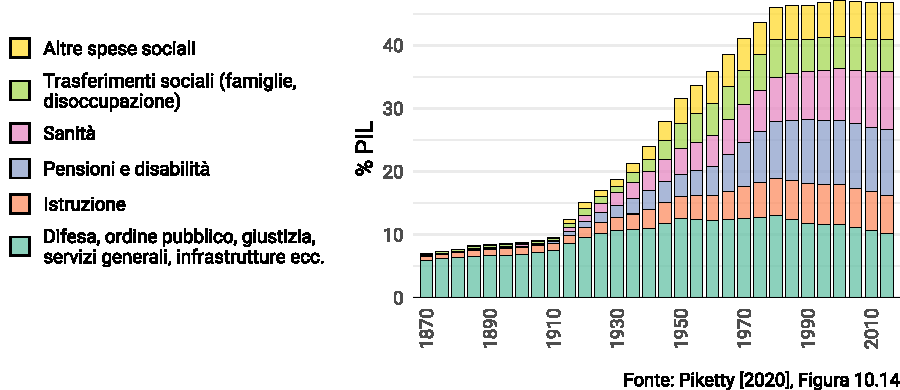
\includegraphics[height=5cm]{./figure/evoluzione-spesa-Piketty-color.pdf}
\end{center}
\vspace{-3mm}

\begin{itemize}
\item La componente che è cresciuta maggiormente nel XX secolo è la spesa sociale (aumentata fino agli anni ‘70, stabilizzata e in alcuni casi diminuita dagli anni '80).
\end{itemize}
\end{frame}

%%%%%%%%%%%%%%%%%%%%%%%%%%%%%%%%%%%%%%%%%%%%
\begin{frame}{Quale dovrebbe essere il ruolo dello Stato?}
\begin{itemize}
\item Abbiamo analizzato l’evoluzione della spesa pubblica e del ruolo dello Stato in ottica \alert{positiva}.
\item Da un punto di vista \alert{normativo}, possiamo chiederci quale «dovrebbe essere» tale ruolo.
  \begin{itemize}
  \item Possiamo individuare una dimensione ottimale?
  \item Esiste un criterio per stabilire cosa debba essere gestito dal pubblico e cosa lasciato all’iniziativa privata (al mercato)?
\end{itemize}
\item Anche la riflessione sul «dover essere» si è evoluta, seguendo l’evoluzione \emph{di fatto} del ruolo dello Stato, risentendo dei mutamenti storici e dell’evoluzione della riflession economica, filosofica, giuridica ecc.
\end{itemize}
\end{frame}

%%%%%%%%%%%%%%%%%%%%%%%%%%%%%%%%%%%%%%%%%%%%
\begin{frame}{Il \emph{laissez-faire} di Adam Smith}
\begin{itemize}
\item Nella visione del \alert{liberalismo economico classico}, la ricchezza nazionale è assicurata dal libero interagire degli individui che perseguono il proprio egoistico interesse. L’interferenza dello Stato non condurrà in generale a esiti migliori di quelli che possono essere garantiti dalla \alert{«mano invisibile»} del mercato concorrenziale
\item Tuttavia lo Stato deve garantire alcune funzioni di base:

\begin{quoting}
\fontsize{10}{11}\selectfont
«In primo luogo, il compito di proteggere la società dalla violenza e l’invasione delle altre società indipendenti; in secondo luogo, il compito di proteggere, per quanto è possibile, ciascun membro della società dall’ingiustizia e dall’oppressione di ogni altro membro di essa, ovvero il dovere di stabilire una rigorosa giustizia; in terzo luogo, il compito di realizzare e mantenere certi lavori pubblici e certe istituzioni pubbliche la cui realizzazione e mantenimento non saranno mai nell’interesse di un individuo o un piccolo gruppo di individui, dal momento che i profitti non potrebbero mai ripagare le spese sostenute da un individuo o un piccolo gruppo di individui, benché possano più che ripagarle a una grande società.»
\end{quoting}
\end{itemize}
\end{frame}

%%%%%%%%%%%%%%%%%%%%%%%%%%%%%%%%%%%%%%%%%%%%
\begin{frame}{Il liberalismo oltre lo «stato minimo»: John Stuart Mill}
\begin{itemize}
\item J. S. Mill (1806-1873) Mantiene il giudizio favorevole all’azione del mercato rispetto al controllo pubblico:
\begin{quoting}
\fontsize{10}{11}\selectfont
«Nelle società più progredite la grande maggioranza delle cose sono compiute peggio con l’intervento del governo, di come gli individui più interessati alla questione le farebbero, o le farebbero fare, se lasciati a se stessi..»
\end{quoting}
\item Tuttavia, questo giudizio è temperato dalla considerazione di circostanze nelle quali un’azione dello Stato è desiderabile:
\begin{itemize}
\item quando l’individuo non è un buon giudice del proprio interesse;
\item quando il mercato è opera in condizioni di monopolio;
\item quando è necessaria un’azione collettiva coordinata;
\item attività che i privati non hanno interesse a realizzare (infrastrutture, esplorazioni scientifiche, nonché il mantenimento di una «classe colta»).
\end{itemize}
\end{itemize}
\end{frame}

%%%%%%%%%%%%%%%%%%%%%%%%%%%%%%%%%%%%%%%%%%%%
\begin{frame}{Liberisti e interventisti}
\begin{itemize}
\item Nel corso del XX secolo il confronto si mantiene vivace.:
\item Sul fronte che si oppone all’intervento pubblico molti economisti che si rifanno al liberalismo classico («liberisti» è il termine italiano che indica il liberalismo economico)
\begin{itemize}
\item la «scuola austriaca» di von Mises e von Hayek vede nella tendenza ad ampliare l’intervento pubblico una minaccia alla libertà individuale.
\end{itemize}
\item A giustificare l’intervento dello Stato concorre l’opera di J. M. Keynes, che con la sua \emph{Teoria generale} sostiene la necessità di opporsi alle fasi di recessione con programmi di spesa pubblica.
\item L’economia del benessere (A.C. Pigou) teorizza la necessità di un’azione correttiva nei casi in cui gli interessi privati e quelli pubblici divergono (esternalità).
\end{itemize}
\end{frame}

%%%%%%%%%%%%%%%%%%%%%%%%%%%%%%%%%%%%%%%%%%%%
\begin{frame}{Le funzioni dello Stato secondo Musgrave}
\begin{itemize}
\item Secondo Richard Musgrave le funzioni dello Stato sono riconducibili alla seguente tripartizione:
\begin{itemize}
\item \alert{Funzione allocativa}: assicurarsi che adeguate risorse siano destinate a beni e servizi che la società ritiene desiderabili e che il mercato non fornirebbe in misura o qualità sufficiente;
\item \alert{Funzione distributiva}: il perseguimento di un’allocazione dei beni e servizi tra gli individui della collettività che sia «equa» o «giusta»;
\item \alert{Funzione di stabilizzazione}: le politiche macroeconomiche finalizzate a garantire la piena occupazione delle risorse, la stabilità dei prezzi e la crescita, tenendo conto dei vincoli esterni (bilancia commerciale e bilancia dei pagamenti).
\end{itemize}
\item L’azione pubblica non è vista come un’indebita interferenza con il mercato, come un’attività «improduttiva», bensì come uno strumento appropriato per risolvere problemi che il mercato non sarebbe in grado di affrontare:
\end{itemize}
\begin{quoting}
\fontsize{9.5}{10}\selectfont
«Un’iniziativa di carattere cooperativo intrapresa per risolvere problemi di coesistenza sociale in modo democratico ed equo» (R. Musgrave, 1999)
\end{quoting}
\end{frame}

%%%%%%%%%%%%%%%%%%%%%%%%%%%%%%%%%%%%%%%%%%%%
\begin{frame}{Una visione più pessimista: la \emph{public choice}}
\begin{itemize}
\item Lo Stato è esso stesso un’istituzione nella quale operano individui portatori di molteplici interessi, potrebbe muoversi con obiettivi ben diversi dal pubblico interesse.
\item J. Buchanan, riprendendo anche la tradizione italiana di scienza delle finanze (A. De Viti de Marco, M. Pantaleoni, M. Fasiani, U. Mazzola, F. Ferrara), pone l’attenzione sui processi di formazione delle decisioni pubbliche.
\begin{itemize}
\item J. Buchanan e G. Tullock (1962), \emph{The calculus of consent. Logical Foundations of Constitutional Democracy}.
\end{itemize}
\item Nella visione della \alert{public choice} l’azione dello Stato viene analizzata, con gli strumenti propri dell’analisi economica, come esito dell’interazione tra soggetti che ricercano il proprio tornaconto individuale.
\item L’azione dello Stato è per lo più motivata dall’azione di gruppi di pressione che ne utilizzano l’autorità per ottenere dei vantaggi. L’azione pubblica è spesso più un problema che la soluzione.
\end{itemize}
\end{frame}

%%%%%%%%%%%%%%%%%%%%%%%%%%%%%%%%%%%%%%%%%%%%
\begin{frame}{In conclusione}
\begin{center}
\Large
«non esistono regole sul giusto ruolo dello Stato

che possano essere stabilite mediante

un ragionamento a priori»

(P. A. Samuelson)
\end{center}
\end{frame}
\end{document}